%--------------------------------------------------------------------------------------------------
\section{Clustering Algorithms with Fast Queries}
\label{sec:algorithm}

\newcommand{\leftep}{{\tt left}}
\newcommand{\rightep}{{\tt right}}
\newcommand{\level}{{\tt level}}
\newcommand{\cache}{\texttt{cache}\xspace}
\newcommand{\bspan}{{\tt span}}
\newcommand{\lookup}{{\tt lookup}}
\newcommand{\bunion}{{\tt union}}
\newcommand{\bweight}{{\tt weight}}
\newcommand{\epoch}{{\tt epoch}}

%--------------------------------------------------------------------------------------------------

% In this section we present methods for streaming clustering with a focus on query time. We begin with explaining an algorithm $\ct$ from prior work, and present our ideas while building on this. We suppose that there is one query for every $q$ data points.

This section describes algorithms for streaming clustering with an emphasis on
query time. 
%The first algorithm \cctree improves upon \ct from prior work by
%.... \textbf{XXX - write a quick summary of the algo}

%\input{algo-driver}
%\input{cstree}
\newcommand*{\keyset}{\texttt{keySet}\xspace}
%-----------------------------------------------------------
\subsection{Algorithm $\cctree$: Coreset Tree with  Caching}
\label{sec:cctree}
%-----------------------------------------------------------
The $\cctree$ algorithm uses the idea of ``coreset caching'' to speed up
query processing by reusing coresets that were constructed during prior
queries. In this way, it can avoid merging a large number of coresets at query
time. When compared with $\cstree$, the $\cctree$ algorithm 
is with the same update process ($\ctupdate$), but apply caching
coreset during the query.

%--------------------
\begin{figure*}[tb]
  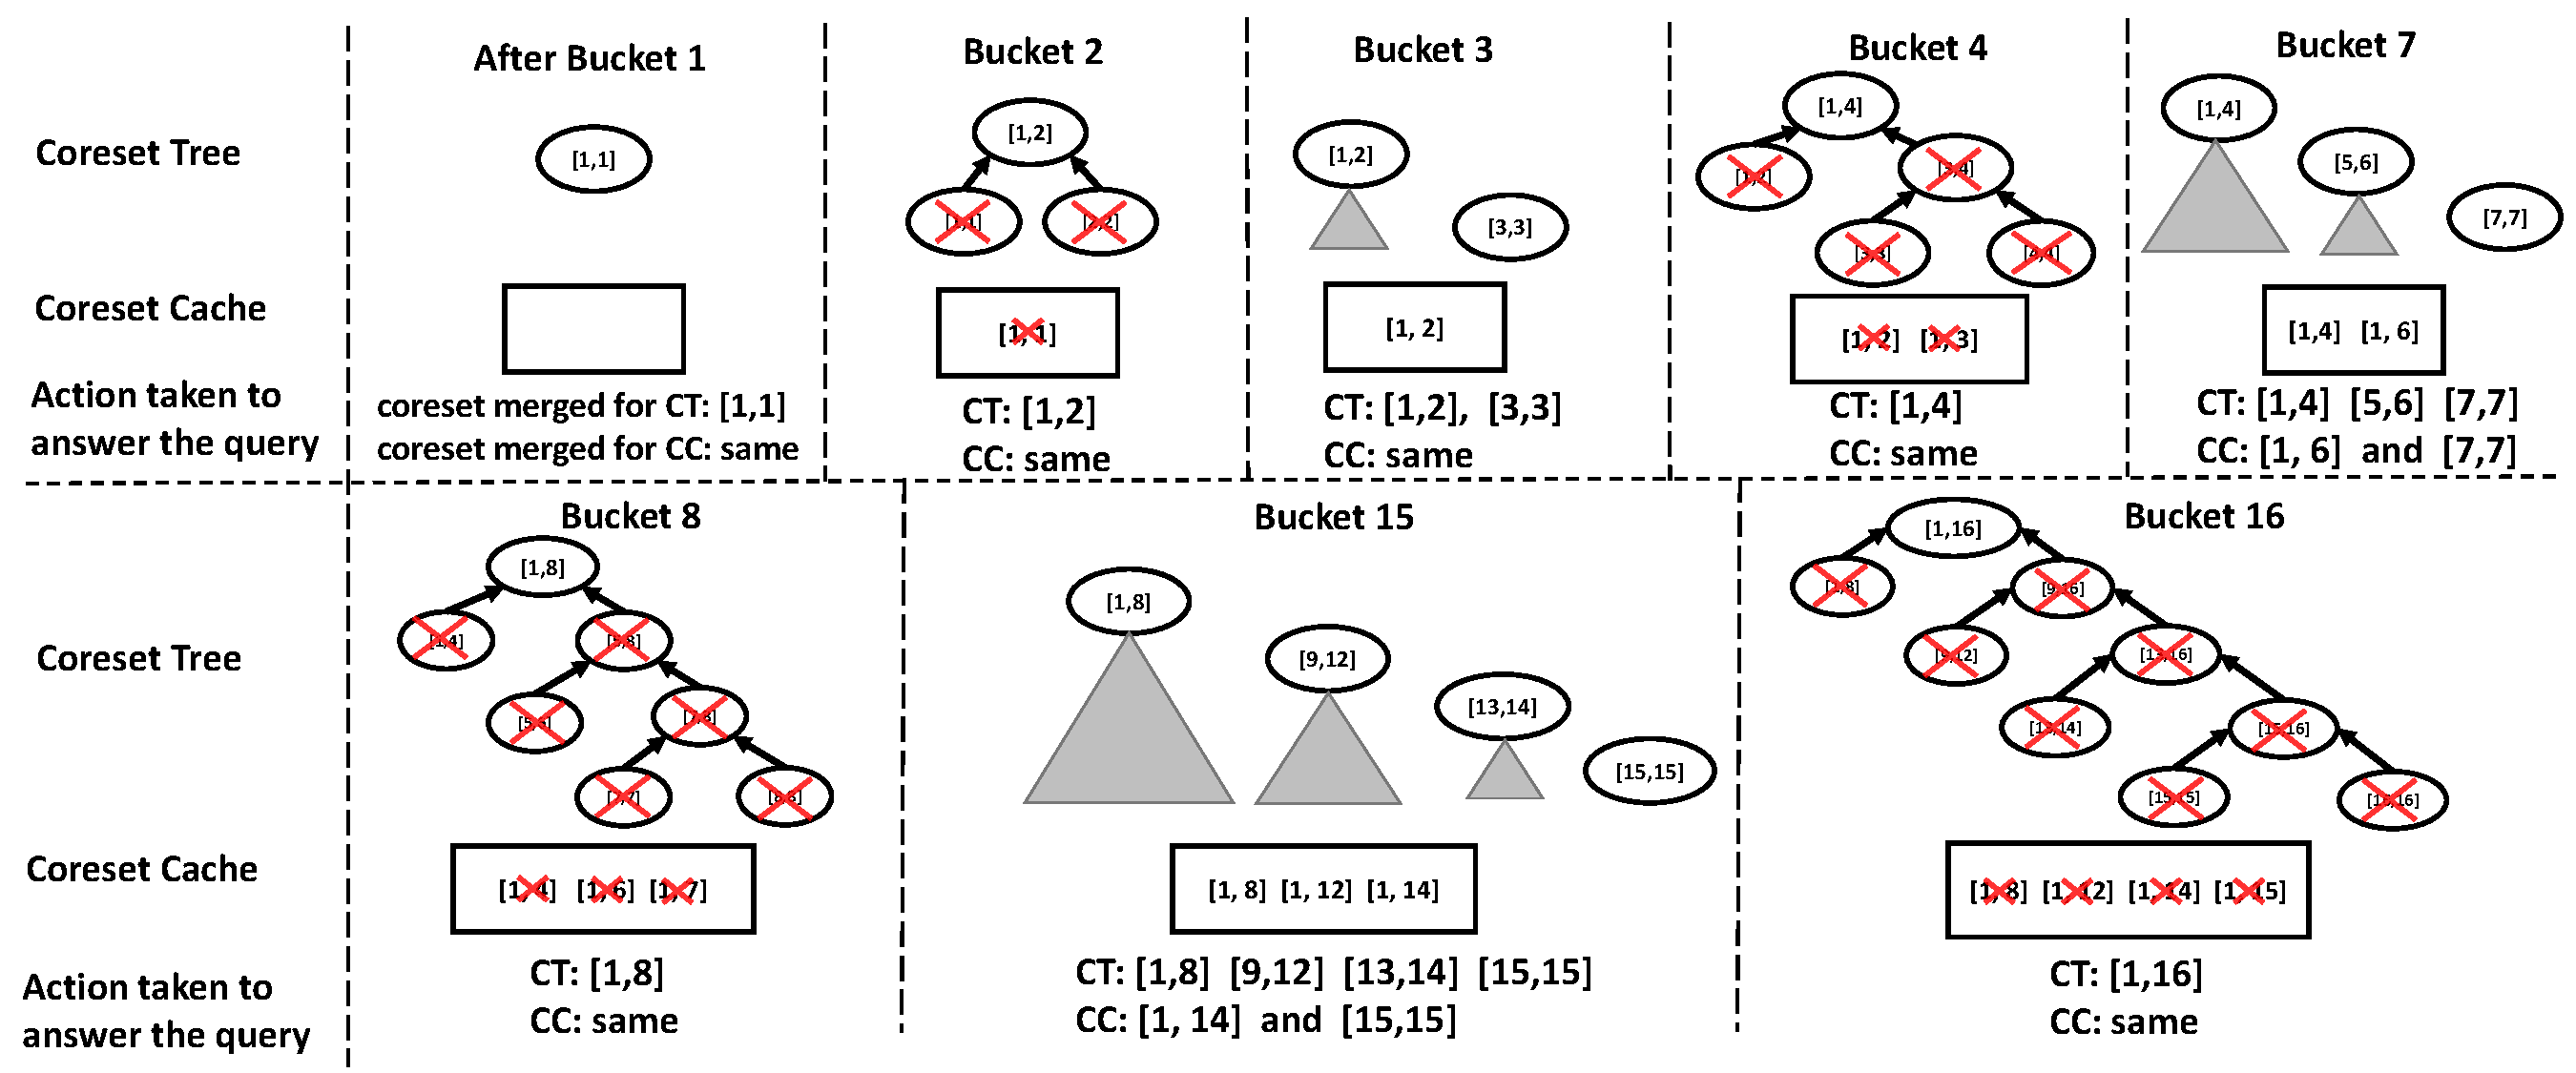
\includegraphics[width=0.98\textwidth]{figs/algo-cc.pdf}
  \caption{Illustration of Algorithm \cc, showing the states of coreset tree and cache after batch $1$, $2$, $3$, $4$, $7$, $8$, $15$ and $16$. The notation $[l,r]$ denotes a coreset of all points in buckets $l$ to $r$, both endpoints inclusive. The coreset tree consists of a set of coresets, each of which is a base bucket or has been formed by merging multiple coresets. Whenever a coreset is merged into a another coreset (in the tree) or discarded (in the cache), the coreset is marked with an ``X''. We suppose that a clustering query arrives after seeing each batch, and describe the actions taken to answer this query (1)~if only \ct was used, or (2)~if \cc was used along with \ct.}
\label{fig:algo-cc}
\end{figure*}
%--------------------

In addition to the coreset tree $\cstree$, the $\cctree$ algorithm
also has an additional \emph{coreset cache} denoted by $\cache$, that stores a
subset of coresets that were previously computed. When a new query has
to be answered, $\cctree$ avoids the cost of merging coresets from
multiple levels in the coreset tree. Instead, it reuses previously
cached coresets and retrieves a small number of additional coresets
which are the same level of the coreset tree, thus leading to less 
computation at query time.

However, the level of the resulting coreset increases linearly with
the number of merges a coreset is involved in. For instance, suppose 
we recursively merge the current coreset with the next arriving base bucket
of coreset to get a new coreset, and so on, for $N$ batches. The resulting 
coreset will have a level of $\Theta(N)$, which can lead to a poor clustering
accuracy. Additional care is needed to ensure that the level of a coreset
is controlled while caching is used.

\noindent\textbf{Details:} Each cached coreset is a summary of base
buckets $1$ through some number $u$. We call this number $u$ as the
\emph{right endpoint} of the coreset and use it as the key/index into
the cache. We call the interval $[1,u]$ as the ``span'' of the
bucket. To explain which coresets can be reused by the algorithm, 
we introduce the following definitions.

%---------------------------------------------
For integers $n > 0$ and $r > 0$, consider the unique decomposition of $n$
according to powers of $r$ as $n = \sum_{i=0}^j \beta_i r^{\alpha_i}$, where
$0 \leq \alpha_0 < \alpha_1 \ldots < \alpha_j$ and $0 < \beta_i < r$ for each
$i$. The $\beta_i$s can be viewed as the non-zero digits in the representation
of $n$ as a number in base $r$. Let $\minor(n,r) = \beta_0 r^{\alpha_0}$, the
smallest term in the decomposition, and $\major(n,r) = n - \minor(n,r)$. Note
that when $n$ is in the form of single term $\beta r^{\alpha}$ 
where $0 < \beta < r$ and $\alpha \geq 0$, $\major(n) = 0$.

For $\kappa =1 \ldots j$, let $n_\kappa = \sum_{i=\kappa}^{j} \beta_i r^{\alpha_i}$. 
$n_\kappa$ can be viewed as the number obtained by dropping the $\kappa$ smallest 
non-zero digits in the representation of $n$ as a number in base $r$. 
The set $\prefixsum(n, r)$ is defined as $\{n_{\kappa} \mid \kappa = 1 \ldots j \}$. 
When $n$ is of the form $\beta r^{\alpha}$ where $0 < \beta < r$, $\prefixsum(n, r)=\emptyset$. 
%---------------------------------------------

For instance, suppose $n=47$ and $r=3$. Since $47 = 1\cdot 3^3 + 2 \cdot 3^2 + 2 \cdot 3^0$, 
we have $\minor(47,3) = 2, \major(47,3) = 45$, and $\prefixsum(47,3) = \{27, 45\}$.

\cc caches every coreset whose right endpoint is in $\prefixsum(N,r)$.
When a query arrives when $N$ buckets received, the task is to compute a coreset
whose span is $[1,N]$. \cc partitions $[1,N]$ as $[1,N_1] \cup [N_1+1,N]$ 
where $N_1 = \major(N,r)$. 
Out of these two intervals, suppose the query comes after every new base bucket received, 
this guarantees that $[1,N_1]$ should be available in the cache. 
$[N_1+1,N]$ is retrieved from the coreset tree, through the union of no more than $(r-1)$ coresets. 
This needs a merge of no more than $r$ coresets. This is in contrast with \ct, 
which may need to merge as many as $(r-1)$ coresets at each level of the tree, 
resulting in a merge of up to $(r-1) \cdot \frac{\log N}{\log r}$ coresets for all levels at query time.

The algorithm for maintaining the cache and answering clustering queries 
is shown in Algorithm~\ref{algo:cctree-functions}. 
The caching process works along with the query process ($\cccoreset$), in a way that
making our algorithm be flexible with the queries by users. When the queries are frequent, 
our algorithm utilizes the cache to provide a faster query speed and a guarantee on the accuracy of 
clustering result. Otherwise in case of the queries are infrequent, we will show that the time complexity 
of updating the cache is at the same level of the query process without caching (algorithm \ct). 
This caching design helps the clustering system to adapt in the faces of both burst queries and occasional queries. 
Figure~\ref{fig:algo-cc} shows an example of how the \cc algorithms updates the cache and answers queries
using cached coresets.

Note that to keep the size of the cache small, as new base buckets arrive,
\ccupdate{} will ensure that ``stale'' or unnecessary coresets are removed. 
The following fact relates to what the cache should store.

%-------------------
\begin{algorithm}
  \caption{Coreset Tree with Caching}
  \label{algo:cctree-functions}
  \label{algo:cctree-init}
  \label{algo:cctree-update}
  \label{algo:cctree-coreset}
\fnDef{$\ccinit(r, k, \eps)$}{
  % Remember the parameters $r$, $k$, and $\eps$.\;
  \tcp{The coreset tree}
  $Q \gets \ctinit{}(r, k, \eps)$ \;
  $\cache \gets \emptyset$
}
\fnDef{$\ccupdate(b,N)$}{
\tcp{$b$ is a new bucket and $N$ is the number of buckets received so far.}
  % Remember $N$\;
  $Q.\ctupdate(b, N)$\;
}
\fnDef{$\cccoreset()$}{
\tcp{Return a coreset of points in buckets $1$ till $N$}
	\uIf{$N$ exists in \cache}
	{
		\Return coreset for buckets $[1, N]$ from the \cache \;
	}
   	$N_1 \gets \major(N,r)$ and $N_2 \gets \minor(N,r)$\;
	Let $N_2=\beta r^{\alpha}$ where $\alpha$ and $\beta < r$ are positive integers\;
	\tcp{coreset for buckets spanning $[1, N_1]$ is not in the \cache}
	\eIf{$N_1$ does not exist in \cache}
	{$U \gets \ctcoreset()$ \;}
	{
		\tcp{$A$ is the coreset for buckets $N_1+1, N_1+2, \ldots, (N_1+N_2)=N$ and is retrieved from the coreset tree}   
   		$a \gets \cup_{B \in Q_\alpha} B$\;
   		\tcp{$b$ is the coreset for buckets spanning $[1, N_1]$, retrieved from the cache} 
   		$b \gets \cache.\lookup(N_1)$ \;
   		$U \gets a \cup b$ \;
   		
	}	
   	\tcp{Store coreset into \cache}
   	%\If{$r$ divides $N$}
   	%{
   		$C \gets \coreset(k, \epsilon, U)$\; 
    	Add coreset $C$ to $\cache$ using key $N$\; 
    	Remove each bucket from $\cache$ whose key does not appear in $\prefixsum(N) \cup \{N\}$  \;
   	%}   
   	\Return {$C$} 
}
\end{algorithm}
%------------------

\begin{fact}
  \label{fact:prefixextension}
  Let $r \geq 2$. For each $N \in \Z^+$,
  $\prefixsum(N+1, r) \subseteq \prefixsum(N,r) \cup \{ N \}$.
\end{fact}
%--------------------------------

Since $\major(N,r) \in \prefixsum(N,r)$ for each $N$, 
if the query comes after each new base bucket received,
we can always retrieve the bucket with span $[1,\major(N,r)]$ from $\cache$.

% -----------------
\begin{lemma}
\label{lemma:cache correctness}
Suppose query comes after receiving each new base bucket. 
Immediately before base bucket $N$ arrives, each $y \in \prefixsum(N,r)$ appears in the key set of \cache.
\end{lemma}
%---------------
\begin{proof}
Proof is by induction on $N$. 
The base case $N=1$ is trivially true, since $\prefixsum(1,r)$ is empty set. 
For the inductive step, assume that before bucket $N$ arrives, 
each $y \in \prefixsum(N, r)$ appears in $\cache$. 
During the query after receiving bucket $N$, 
we store the coreset whose span is $[1, N]$ to the cache.
By Fact~\ref{fact:prefixextension}, we know that
$\prefixsum(N+1, r) \subseteq \prefixsum(N,r) \cup \{N\}$. 
Using this, every bucket with a right endpoint in $\prefixsum(N+1,r)$ 
is present in $\cache$ at the beginning of bucket $(N+1)$ arrives. 
Hence, the inductive step is proved.
\end{proof}
%-----------------

When the queries come less frequent, the cache is less frequently updated as well. 
Then it can not guarantee that the \major is in the cache, that is $N_1$ may not 
exist in the \cache. In this case, the $\cccoreset$ will switch back to the $\ctcoreset$ method in \ct. 
We analyze the time complexity of algorithm $\cc$ under the assumption that we can always use cache 
to accelerate the current query. In practice, we run experiments to show the result of 
algorithm performance when less frequent queries.

%-----------------
\begin{lemma}
\label{lemma:cctree-level}
When queried after inserting base bucket $N$, Algorithm~\cccoreset returns a coreset 
whose level in no more than $\left\lceil 2 \log_r N \right\rceil - 1$.
\end{lemma}
%-----------------
\begin{proof}
Let $\chi(N)$ denote the number of non-zero digits in the representation of $N$ as a number in base $r$. 
We show that the level of the coreset returned by Algorithm~\cccoreset is no more than 
$\left\lceil \log_r N \right\rceil + \chi(N)-1$. 
Since $\chi(N) \le \left\lceil \log_r N \right\rceil$, the lemma follows.

The proof is by induction on $\chi(N)$. If $\chi(N)=1$, then $\major(N,r)=0$,
and the coreset is retrieved directly from the coreset tree $Q$. 
By Fact~\ref{fact:cstree-fact}, each coreset in $Q$ is at a level 
no more than $\lceil \log_r N \rceil$, and the base case follows. 
Suppose the claim was true for all $N$ such that $\chi(N) = t$. Consider $N$ such that
$\chi(N)=(t+1)$. The algorithm computes $N_1 = \major (N,r)$, and retrieves the
coreset with span $[1,N_1]$ from the cache. Note that $\chi(N_1) = t$. By the
inductive hypothesis, the coreset for span $[1,N_1]$ is at a level
$\left\lceil \log_r N \right\rceil + t - 1$. The coresets for span
$[N_1+1,N]$ are retrieved from the coreset tree; note there are multiple such
coresets, but each of them is at a level no more than
$\left\lceil \log_r N \right\rceil$, using Fact~\ref{fact:cstree-fact}.  
The level of the union coreset for span $[1,N]$ is no more than
$\left\lceil \log_r N \right\rceil + t$, proving the inductive case.
\end{proof}
%-----------------

With the coreset level bounded, we can give the guarantee on the accuracy of clustering centers.
Let the accuracy parameter $\eps=\frac{c \log r}{2\log N}$, where $c < \ln{1.1}$.
%-----------------
\begin{lemma}
\label{lemma:cctree-accuracy}
After observing $N$ buckets from the stream, when using clustering data structure \cc, 
Algorithm~\clusterquery returns a set of $k$ points whose clustering cost 
is within a factor of $O(\log k)$ of the optimal $k$-means clustering cost.
\end{lemma}
%-----------------
\begin{proof}
The proof is similar as Lemma~\ref{lemma:cstree-accuracy}. From Lemma~\ref{lemma:cctree-level}, 
we know that the level of a coreset returned is no more than $\left\lceil 2 \log_r N \right\rceil - 1$. 
Using Lemma~\ref{lemma:cstree-level2}, the returned coreset, say $C$, is an $\eps'$-coreset where 
$\eps' = \left[ \left(1 + \frac{{c}\log r}{2\log N}\right)^{\frac{2\log N}{\log r}} - 1 \right] \le \left[ e^{\left(\frac{{c}\log r}{2\log N}\right) \cdot \frac{2\log N}{\log r}}-1 \right] < 0.1$.
Following an argument similar to that of Lemma~\ref{lemma:cstree-accuracy}, we arrive at the result.
\end{proof}
%----------------------

The following lemma shows the time and space complexity of the \cache. 
We show that the time on updating the \cache is at least at the same level of 
the time of answering a query in Algorithm~$\ct$, and can be better to be in linear
scale of $r$ instead of $\frac{r \log N}{\log r}$.
%-----------------------
\begin{lemma}
\label{lemma:cctree-time}
Algorithm~\ref{algo:cctree-update} processes a stream of points 
using amortized time $O(dm)$ per point, 
using memory of $O\left(dm \cdot \frac{r \log N}{\log r} \right)$. 
The amortized cost of answering a query is $O\left(\frac{kdm}{q} \cdot r \right)$.
\end{lemma}
%-----------------

%-----------------
\begin{proof}
The runtime for Algorithm~\ccupdate~ is same as the Algorithm~\ctupdate. 
The update time for \ccupdate is $O(dm)$ per point.

From Lemma~\ref{lemma:cache correctness}, $N_1$ is always in the \cache. 
Algorithm~\cccoreset combines no more than $r$ buckets, 
out of which there is no more than one bucket from the cache, 
and no more than $(r-1)$ from the coreset tree. 
From Theorem~\ref{theo:coreset-build}, the time to compute coreset 
on $O(mr)$ points is $O(d m^2 r)$, and coreset size $m$ is $O(k)$.
The time to compute coreset $C$ is $O(kdmr)$.   
To compute the $k$ centers from $U$, 
it is necessary to run $\kmpp$ on $O(mr)$ points using time $O(kdmr)$. 
The amortized query time per point is $O\left( \frac{kdmr}{q} \right)$.

\remove {
In the worst case, when the major part is always not in the cache. 
Comparing to Algorithm~\ct, the additional time cost is updating the cache. 
The number of points in set $U$ is at most $(m \cdot \frac{r \log N}{\log r})$, 
computation time is $O(d m^2 r \cdot \log_r N)$. 
As the size of coreset is $O(k)$, 
the addition time for constructing coreset is $O(kdm \cdot \frac{r \log N}{\log r})$ 
at the same level of the query time by \ct.
}

The coreset tree $Q$ uses space $O\left( dm \cdot \frac{r \log N}{\log r} \right)$. 
After processing bucket $N$, $\cache$ only stores those buckets that are 
corresponding to $\prefixsum(N,r) \cup \{ N \}$. 
The number of such buckets possible is $O(\log_r N )$, 
so the space cost of $\cache$ is $O(dm \cdot \frac{\log N}{\log r})$. 
The space complexity follows.
\end{proof}
%-----------------


\subsection{Algorithm $\rcc$: Recursive Coreset Cache}
\newcommand{\rmax}{\rho}
\newcommand{\order}{\texttt{order}}
\newcommand{\mainds}{\mathcal{R}}

There are still a few issues with the $\cc$ data structure. First, the level of
the coreset finally generated is $O(\log_rN)$. Since theoretical guarantees on
the approximation quality of clustering worsen with the number of levels of the
coreset, it is natural to ask if the level can be further reduced to $O(1)$.
Moreover, the time taken to process a query is linearly proportional to $r$; we
wish to reduce the query time even more.  While it is natural to aim to
simultaneously reduce the level of the coreset as well as the query time, at
first glance, these two goals seem to be inversely related. It seems that if we
decreased the level of a coreset (better accuracy), then we will have to
increase the merge degree, which would in turn increase the query time. For
example, if we set $r=\sqrt{N}$, then the level of the resulting coreset is
$O(1)$, but the query time will be $O(\sqrt{N})$.

In the following, we present a solution $\rcc$ that uses the idea of coreset
caching in a recursive manner to achieve both a low level of the coreset, as
well as a small query time. In our approach, we keep the merge degree $r$ 
in a relatively high value, thus keeping the levels of coresets low. 
At the same time, we use coreset caching even within a single level of a coreset tree, 
so that there is no need to merge $r$ coresets at query time. 
Special care is required for coreset caching in this case, 
so that the level of the coreset does not increase significantly.

For instance, suppose we built another coreset tree with merge degree $2$ for
the $O(r)$ coresets within a single level of the current coreset tree, this
would lead to a inner tree with level of $\log r$. At query time, we aggregate
$O(\log r)$ coresets from this inner tree, in addition to a coreset from the \cc. So, this will lead to a level of $O\left(\max\left\{\frac{\log N}{\log r}, \log r\right \}\right)$ and a query time proportional to $O(\log r)$. This is an improvement from the coreset cache, which has a query time proportional to $r$ and a level of $O\left(\frac{\log N}{\log r}\right)$.

We can take this idea further by recursively applying the same idea to the
$O(r)$ buckets within a single level of the coreset tree. Instead of having a
coreset tree with merge degree $2$, we use a tree with a higher merge degree,
and then have a coreset cache for this tree to reduce the query time, and apply
this recursively within each tree. This way we can approach the ideal of a small
level and a small query time. We are able to achieve interesting tradeoffs, as
shown in Table~\ref{table:rcc}. To keep the level of the resulting coreset low,
along with the coreset cache for each level, we also maintain a list of coresets
at each level, like in the $\ct$ algorithm. To merge coresets to a higher level,
we use the list, rather than the recursive coreset cache.

More specifically, the $\rcc$ data structure is defined inductively as
follows. For integer $i \ge 0$, the $\rcc$ data structure of order $i$ is
denoted by $\rcc(i)$. $\rcc(0)$ is a $\cctree$ data structure with a merge
degree of $r_0 = 2$. For $i>0$, $\rcc(i)$ consists of:
%-----------------
%\begin{itemize}[topsep=-0.5em,leftmargin=*, itemsep=2pt]
\begin{itemize}
\item $\cache(i)$, a coreset cache storing previous coresets.

\item For each level $\ell = 0, 1, 2, \ldots$, there are two structures. 
One is a list of buckets $L_{\ell}$, 
similar to the structure $Q_{\ell}$ in a coreset tree. 
The maximum length of a list is $r_{i} = 2^{2^i}$. 
Another is an $\rcc_{\ell}$ structure which is a $\rcc$ 
structure of a lower order $(i-1)$, which stores the same information as list $L_\ell$, 
except in a way that can be quickly retrieved during a query.
\end{itemize}
%-----------------

The main data structure $\mainds$ is initialized as $\mainds = \rccinit(\iota)$, 
for a parameter $\iota$, to be chosen. 
Note that $\iota$ is the highest order of the recursive structure. 
This is also called the ``nesting depth" of the structure. 

%-----------------
\begin{algorithm}[t]
\DontPrintSemicolon
\caption{$\mainds.\rccinit(\iota)$
\label{algo:rcc-init}
}
$\mainds.\order \gets \iota$, 
$\mainds.\cache \gets \emptyset$, 
$\mainds.r \gets 2^{2^{\iota}}$\;

\tcp{$N$ is the number of buckets so far}
$\mainds.N \gets 0$\; 
\ForEach{$\ell=0,1,2, \ldots$}
{
   $\mainds.L_{\ell} \gets \emptyset$\;
   \uIf{$\mainds.\order > 0$}
   {$\mainds.\rcc_{\ell} \gets \mainds.\rccinit(\mainds.\order - 1)$}
}
\Return $\mainds$\;
\end{algorithm}
%-----------------

%-----------------
\begin{algorithm}[t]
\DontPrintSemicolon
\caption{$\mainds.\rccupdate(b)$
\label{algo:rcc-update}}
\tcp{$b$ is a new base bucket}
$\mainds.N \gets \mainds.N + 1$\;
\tcp{Insert $b$ into $\mainds.L_0$ and merge if needed}
Append $b$ to $\mainds.L_0$.\;
\If{$\mainds.\order > 0$} 
{
	recursively update $\mainds.\rcc_0$ by $\mainds.\rcc_0.\rccupdate(b)$ \;
}
\;
\tcp{Clear $\mainds.L$ and $\rcc$ if number of buckets reaches $r$}
$\ell \gets 0$\;
\While{$(|\mainds.L_\ell| = \mainds.r)$}
{
  %$b' \gets$ {\tt BucketMerge}($\mainds.L_\ell$)\;
  $b' \gets \coreset(k, \eps, \cup_{B \in \mainds.L_\ell} B)$ \;
  Append $b'$ to $\mainds.L_{\ell+1}$ \;
  \If{$\mainds.\order > 0$}
  {recursively update $\mainds.\rcc_{\ell+1}$ by $\mainds.\rcc_{\ell+1}.\rccupdate(b)$} \;
  \tcp{Empty the list of coresets $\mainds.L$}
  $\mainds.L_{\ell} \gets \emptyset$ \;
  \tcp{Empty the \rcc structure}
  \If{$\mainds.\order > 0$} 
  {$\mainds.\rcc_{\ell} \gets \rccinit(\mainds.\order-1)$} \;
  $\ell \gets \ell + 1$ \;
}
\end{algorithm}
%-----------------

%------------------
\begin{algorithm}[t]
\DontPrintSemicolon
\caption{
$\mainds.\rcccoreset()$
\label{algo:rcc-getbuckets}
\label{algo:rcc-coreset}
}
$U \gets \emptyset$ \;
$N_1 \gets \major(\mainds.N, \mainds.r)$ \;
\eIf{$N_1$ does not exist in $\mainds.\cache$} 
{
	$U \gets \cup_{\ell} \{ \mainds.\rcc_{\ell}.\rcccoreset() \}$ \;
}
{
	$b_1 \gets$ retrieve coreset with endpoint $N_1$ from $\mainds.\cache$\;
	Let $\ell^*$ be the lowest numbered non-empty level among $\mainds.L_i, i \ge 0$.\;
	\tcp{Apply $\rcc$ data structure to retrieve the coresets from level $\ell^*$}
	\eIf{$\mainds.\order > 0$}
	{$b_2 \gets \mainds.\rcc_{\ell^*}.\rcccoreset()$}
	{$b_2 \gets \mainds.L_{\ell^*}$}
	$U \gets b_1 \cup b_2$ 
}

\tcp{Store coreset into \cache}
%\If{$\mainds.r$ divides $\mainds.N$}
%{
	$b' \gets \coreset(k, \epsilon, U)$\;
	Add $b'$ to $\mainds.\cache$ with right endpoint $\mainds.N$\;
	From $\mainds.\cache$, remove all buckets $b''$ such that 
	$\rightep(b'') \notin \prefixsum(\mainds.N) \cup \{ N \}$ \;
%}
\Return $b'$
\end{algorithm}
%-----------------

%-----------------
\begin{table}[ht]
{
\footnotesize
\setlength{\tabcolsep}{2pt}
\begin{tabular}{ c c c c c}
\toprule
$\iota$ & coreset level & Query cost  & update cost & Memory \\
        & at query      & (per point) & per point   & \\
\midrule
$\log \log N - 3$ & $O(1)$ & $O\left( \frac{kdm}{q} \log \log N \right)$ & $O(dm \log \log N)$ & $O\left( dmN^{1/8} \right)$ \\
\midrule
$\log \log N / 2$ & $O(\sqrt{\log N})$ & $O \left( \frac{kdm}{q} \log \log N \right)$ & $O(dm \log \log N)$ & $O \left( dm 2^{\sqrt{\log N}} \right)$ \\
\bottomrule
\end{tabular}
\smallskip
\caption{Possible tradeoffs for the $\rcc(\iota)$ algorithm, based on the parameter $\iota$, the nesting depth of the structure.
\label{table:rcc}}
}
\end{table}
%-----------------

%-----------------
\begin{lemma}
\label{lemma:rcc-level}
When queried after inserting $N$ buckets, 
Algorithm~\ref{algo:rcc-coreset} using $\rcc(\iota)$ returns a coreset 
whose level is $O\left(\frac{\log N}{2^{\iota}}\right)$. 
The amortized time cost of answering a clustering query is 
$O\left(\frac{kdm}{q} \cdot \log \log N \right)$ per point. 
\end{lemma}
%-----------------
\begin{proof}
Algorithm~\ref{algo:rcc-coreset} retrieves a few coresets from $\rcc$ of different orders. 
From the outermost structure $\rcc(\iota)$, 
it retrieves one coreset $c$ from $\cache(\iota)$. 
Using an analysis similar to Lemma~\ref{lemma:cctree-level}, 
the level of $b_{1}$ is no more than $\frac{2 \log N}{\log r_{\iota}}$. 

Note that for $i < \iota$, the maximum number of coresets that will be inserted
into $\rcc(i)$ is $r_{i+1} = r_i^2$. The reason is that inserting $r_{i+1}$
buckets into $\rcc(i)$ will lead to the corresponding list structure for
$\rcc(i)$ to become full. At this point, the list and the $\rcc(i)$ structure
will be emptied out in Algorithm~\ref{algo:rcc-update}. From each recursive call
to $\rcc(i)$, it can be similarly seen that the level of a coreset retrieved
from the cache is at level $\frac{2 \log{r_i}}{\log r_{i-1}}$, which is
$O(1)$. The algorithm returns a coreset formed by the union of all the coresets,
followed by a further merge step. Thus, the coreset level is one more than the
maximum of the levels of all the coresets returned, which is
$O\left( \frac{\log N}{\log r_{\iota}} \right)$.

For the query cost, similar to our analysis in $\cc$, we assume that 
for each order of $\rcc(i)$, we can always use the cache in coreset queries.
Comparing to Algorithm~\cccoreset, the minor part of coreset is retrieved from the inner 
\rcc data structure with lower order. Thus, for each order of $\rcc$, the number 
of coresets merged is $2$. The number of coresets merged at query time 
is equal to two times the nesting depth of the structure, that is $2 \cdot \iota$. 
The query time equals the cost of running $\kmpp$ on the union of all these coresets, 
for a total time of $O(kd m \log \log N)$. The amortized per-point cost of a query follows.

\remove{
Consider the case that the coreset of major does not exist in the cache. 
Suppose all the caches at different order are not available, our algorithm 
uses \ctcoreset to retrieve coresets at each order of \rcc. 
Note that the number of levels for each $\rcc(i)$ is at most $2$ except the $\rcc(\iota)$. 
The reason is as follows. 
It is necessary to insert $r_{i+1} = r_i^2$ buckets into $\rcc(i)$. 
Since this is the maximum number of buckets that will be inserted into $\rcc(i)$, 
there are at most two levels of lists within each $\rcc(i)$ for $i < \iota$.
The number of coresets be merged for $\rcc(\iota-1)$ is $2^{\iota-1}$, which is $O(\log r_{\iota})$.
The total number of coresets be merged is 
$O\left( \frac{\log N}{\log r_{\iota}} \cdot \log r_{\iota} \right) = O(\log N)$, 
and query time is $O(kd m \log N)$.
}
\end{proof}
%-----------------


%-----------------
\begin{lemma}
\label{lemma:rcc-performance}
The memory consumed by $\rcc(\iota)$ is $O(dm r_{\iota})$. 
The amortized processing time is $O(dm \log \log N)$ per point.
\end{lemma}
%-----------------
\begin{proof}
First, as stated in the proof of Lemma~\ref{lemma:rcc-level}, 
in $\rcc(i)$ for $i < \iota$, there are at most two level of lists $L_{\ell}$. 

%First, we note in $\rcc(i)$ for $i < \iota$, there are $O(1)$ lists $L_{\ell}$.
%The reason is as follows. 
%It can be seen that in order to get a single bucket in list $L_2$ within $\rcc(i)$, 
%it is necessary to insert $r_i^2=r_{i+1}$ buckets into $\rcc(i)$. 
%Since this is the maximum number of buckets that will be inserted into $\rcc(i)$, 
%there are no more than three levels of lists within each $\rcc(i)$ for $i < \iota$. 

We prove by induction on $i$ that $\rcc(i)$ has no more than $6r_i$ buckets.  
For the base case, $i=0$, and we have $r_0=2$. 
In this case, $\rcc(0)$ has two levels, each with no more than $2$ buckets. 
So that the total memory is no more than $6$ buckets, due to the lists in two levels, 
and no more than $2$ buckets in the cache, for a total of $6=3r_0 < 6r_0$ buckets. 
For $i=1$,  $r_1=4$, the two lists have at most $8$ buckets and cache has no more than $2$ buckets. 
The recursive structures $\rcc(0)$ has $6$ buckets and there are two recursive structures, one for each level. 
Thus in total $\rcc(1)$ has no more than $22$ buckets, which is less than $24 = 6r_1$ buckets. 

For the inductive case, consider that $\rcc(i)$, the list at each level has no more than $r_i$ buckets. 
The recursive structures $\rcc_{\ell}$ within $\rcc(i)$ themselves have no more than $6r_{i-1}$ buckets. 
Adding the constant number of buckets within the cache, 
we get the total number of buckets within $\rcc(i)$ to be 
$2r_i + 2 \cdot 6r_{i-1} + 2 = 2r_i + 12 \sqrt{r_i} + 2 \le 6 r_i$, 
for $r_i \ge 16$, i.e. $i \ge 2$. 
Thus if $\iota$ is the nesting depth of the structure, 
the total memory consumed is $O(dm r_{\iota})$, since each bucket requires $O(dm)$ space.

For the updating process time cost, when a bucket is inserted into $\mainds = \rcc(\iota)$, 
it is added to list $L_0$ within $\mainds$. 
The cost of maintaining these lists, 
that is the cost of merging into higher level lists, 
is amortized $O(dm)$ per point, 
similar to the analysis in Lemma~\ref{lemma:cctree-time}. 
The bucket is also recursively inserted into a $\rcc(\iota-1)$ structure, 
and a further structure within, 
and the amortized time for each such structure is $O(dm)$ per point. 
The total time cost is $O(dm\iota)$ per point which is equal to $O(dm \log \log N)$.
\end{proof}
%-----------------

Different tradeoffs are possible by setting $\iota$ to specific values. Some examples are shown in the Table~\ref{table:rcc}.

\newcommand{\fallbackcost}{\texttt{$\phi_{prev}$}\xspace}
\newcommand{\estcost}{\texttt{$\phi_{now}$}\xspace}

%---------------------------
\subsection{Online Coreset Cache: a Hybrid of \cc and \seqkm}
\label{sec:hybrid}
%---------------------------

%--------------------
\begin{figure}[t]
  	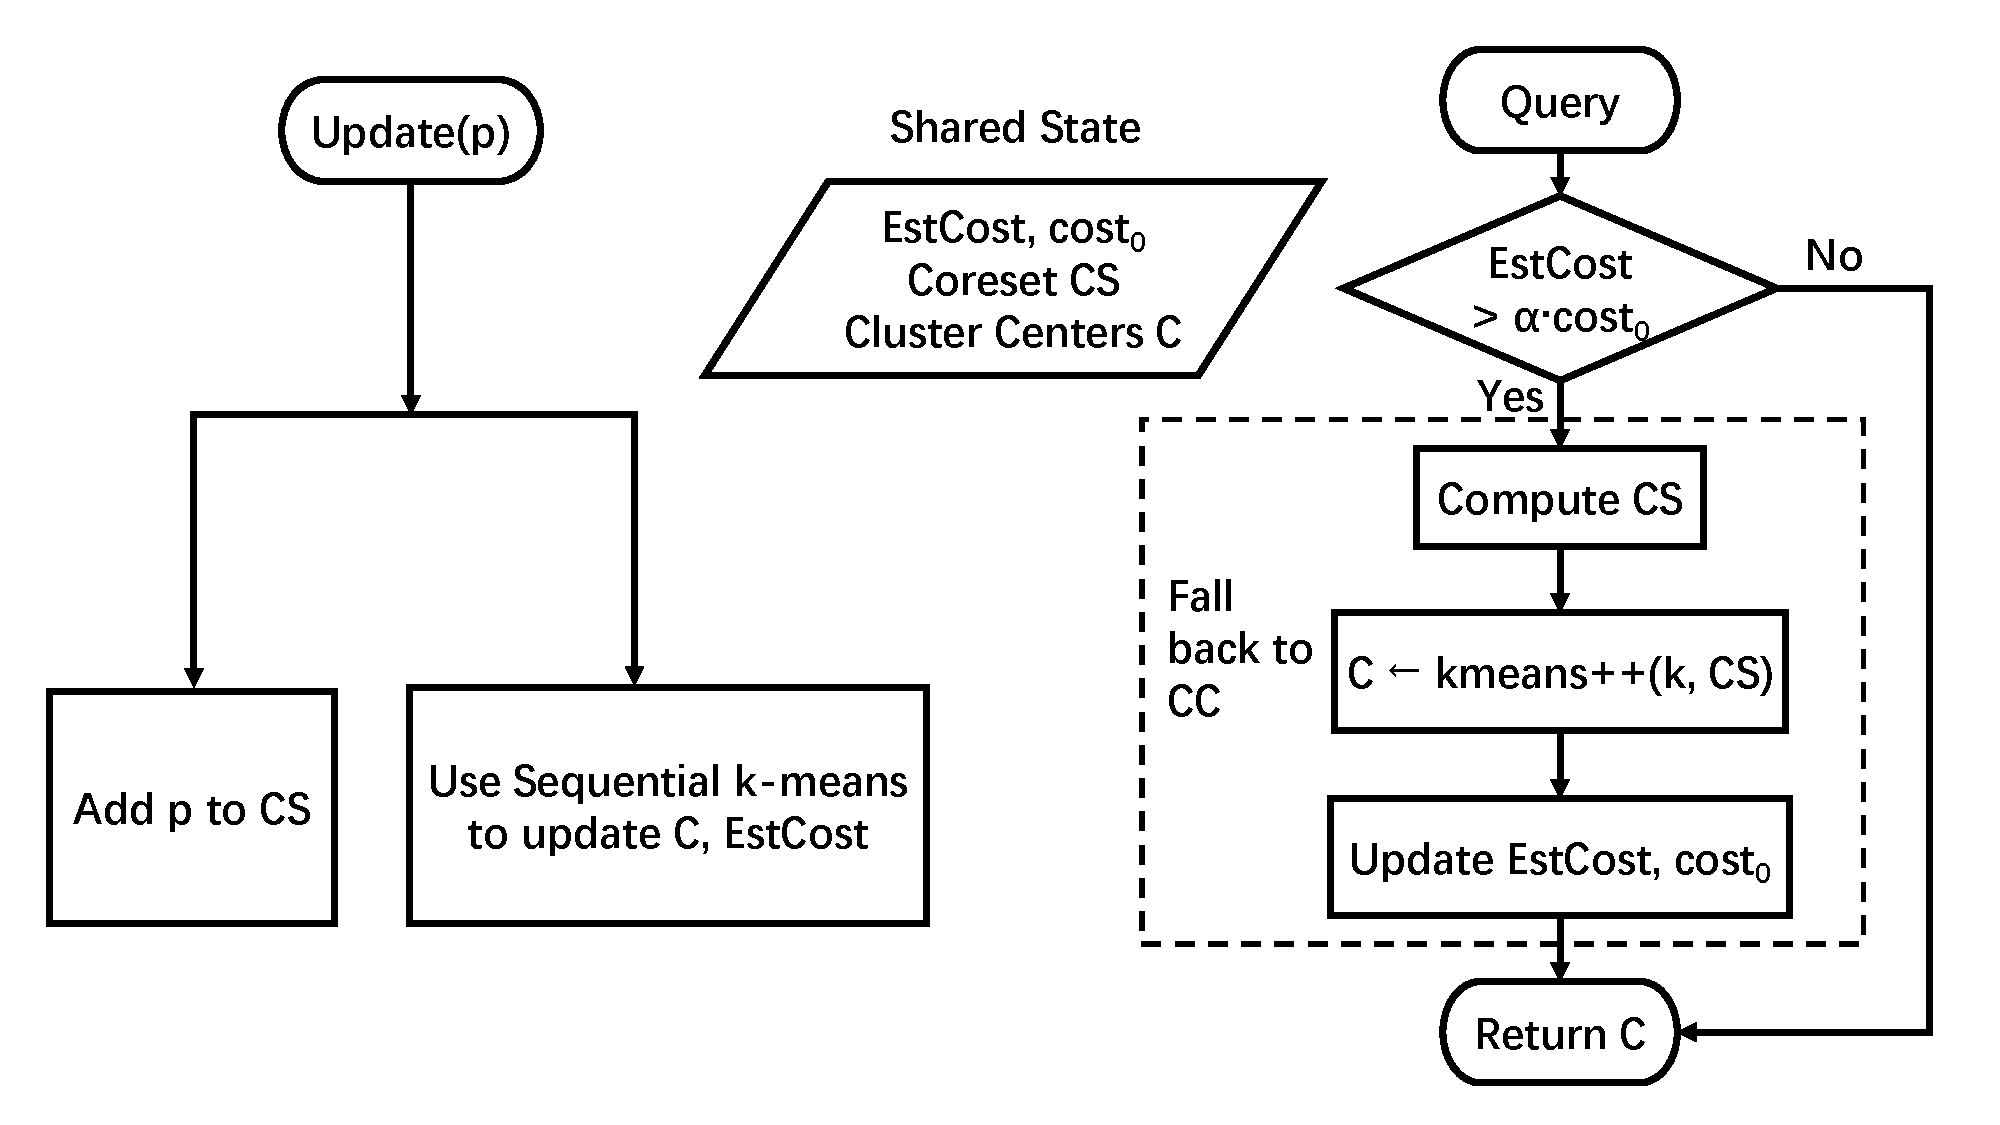
\includegraphics[width=0.49\textwidth]{figs/algo-onlinecc.pdf}
  	\caption{Illustration of Algorithm \hybrid.}
\label{fig:algo-onlinecc}
\end{figure}
%--------------------

If we break down the query runtime of the algorithms considered so far, we
observe two major components: (1)~the construction of the coreset of all points
seen so far, through merging stored coresets; and (2)~the \kmpp algorithm
applied on the resulting coreset. The focus of the algorithms discussed so far (
\cc and \rcc) is on decreasing the runtime of the first component, coreset
construction, by reducing the number of coresets to be merged at query time. But
they still have to pay the cost of the second component \kmpp, which is
substantial in itself, since the runtime of \kmpp is $O(kdm)$, where $m$ is the
size of the coreset. To make further progress, we have to reduce this
component. However, the difficulty in eliminating \kmpp at query time is that
without an approximation algorithm such as \kmpp, we have no way to guarantee
that the returned clustering is an approximation to the optimal.


This section presents an algorithm, \hybrid, which only occasionally runs \kmpp
at query time, and most of the time, uses a much cheaper method that costs
$O(1)$ to compute the clustering centers. \hybrid uses a combination of \cc and
the \seqkm algorithm~\cite{MacQueen67} (aka. Online Lloyd's algorithm) to
maintain the cluster centers quickly while also providing a guarantee on the
quality of clustering. Like \seqkm, it incrementall updates the current set of
cluster centers for each arriving point. However, while \seqkm can process
incoming points (and answer queries) extremely quickly, it cannot provide any
guarantees on the quality of answers, and in some cases, the clustering quality
can be very poor when compared with say, \kmpp. To prevent such deterioration in
clustering quality, our algorithm (1)~occasionally falls back to \cc, which is
provably accurate, and (2)~runs \seqkm so long as the clustering cost does not
get much larger than the previous time \cc was used. This ensures that our
clusters always have a provable quality with respect to the optimal.

To accomplish this, \hybrid also processes incoming points using \cc, thus
maintaining coresets of substreams of data seen so far. When a query arrives, it
typically answers them in $O(1)$ time using the centers maintained using
\seqkm. If, however, the clustering cost is significantly higher (by more than a
factor of $\alpha$ for a parameter $\alpha > 1$) than the previous time that the
algorithm fell back to \cc, then the query processing again returns to \cc to
regenerate a coreset. One difficulty in implementing this idea is that
(efficiently) maintaining an estimate of the current clustering cost is not
easy, since each change in cluster centers can affect the contribution of a
number of points to the clustering cost. To reduce the cost of maintenance, our
algorithm keeps an upper bound on the clustering cost; as we show further, this
is sufficient to give a provable guarantee on the quality of clustering. Further
details on how the upper bound on the clustering cost is maintained, and how
algorithms \seqkm and \cc interact are shown in Algorithm~\ref{algo:hybrid}, 
with a schematic illustration in Figure~\ref{fig:algo-onlinecc}.


%----------------
\begin{algorithm}[t]
\label{algo:hybrid}
\caption{The Online Coreset Cache: A hybrid of \cc and \seqkm algorithms}

\fnDef{$\hybridinit(k, \eps, \alpha)$}{
%Remember coreset approximation factor $\eps$, merge-degree $r$, and parameter $\alpha > 1$ the threshold to switch the query processing to \cc \;

\tcp{$C$ is the current set of cluster centers}
Initialize $C$ by running $\kmpp$ on set $\stream_0$ consisting of the first $O(k)$ points of the stream\;

\tcp{\fallbackcost is the clustering cost during the previous ``fallback'' to \cc; 
\estcost is an estimate of the clustering cost of $C$ on the stream so far}
\fallbackcost , \estcost $\gets$ clustering cost of $C$ on $\stream_0$\;
$Q \gets \ccinit(r,k,\eps)$\;
}

\tcp{On receiving a new point $p$ from the stream}
\fnDef{$\hybridupdate(p)$}{
	Assign $p$ to the nearest center $c_p$ in $C$  \;

    $\estcost \gets \estcost + \edist{p}{c_p}^2$ \;
	
	\tcp{Compute new centroid of $c_p$ and $p$ where $w$ is the weight of $c_p$}
	$c_p'  \gets (w \cdot c_p + p) / (w + 1)$   \; 
	Assign the position of $c_p'$ to $c_p$  \;
    Add $p$ to the current bucket $b$. If $|b|=m$, then $Q.\ccupdate(b)$ \;
}

\fnDef{$\hybridquery()$}{
	\If{$\estcost > \alpha \cdot \fallbackcost$}
	{
	     $CS \gets Q.\cccoreset() \cup b$, where $b$ is the current bucket that not yet inserted into $Q$ \;

             $C \gets \kmpp(k, CS)$   \;
             $\fallbackcost \gets \phi_C(CS)$, the \km cost of coreset $CS$ on centers $C$  \;
             $\estcost \gets \fallbackcost / (1-\eps)$   \;
	}
  \Return $C$  \;
}
\end{algorithm}
%-----------------

We state the properties of Algorithm~\hybrid in Lemma~\ref{lemma:ecost} and ~\ref{lemma:online}.
%----------------
\begin{lemma}
\label{lemma:ecost}
In Algorithm~\ref{algo:hybrid}, after observing point set $P$ from the stream, if $C$ is the current set of cluster centers, then $\estcost$ is an upper bound on $\phi_C(P)$.
\end{lemma}
%---------------
\begin{proof}
Consider the value of $\estcost$ between every two consecutive switches to \cc. Without loss of generality, suppose there is one switch happens at time $0$, let $P_0$ denote the points observed until time $0$ (including the points received at $0$). We will do induction on the number of points received after time $0$, we denote this number as $i$. Then $P_i$ is $P_0$ union the $i$ points received after time $0$. Let $\estcost (i)$ denote the cost $\estcost$ at time $i$. 

When $i$ is $0$, we compute $C$ from the coreset $CS$, from the coreset definition
\[
\fallbackcost = \phi_{C}(CS) \geq (1-\epsilon) \cdot \phi_{C}(P_0)
\] 
where $\epsilon$ is the approximation factor of coreset $CS$. So for dataset $P_0$, 
the estimation cost $\estcost(0) = \fallbackcost / (1-\eps) \geq \phi_{C}(P_0)$.

At time $i$, denote $C_i$ as the cluster centers maintained and $\estcost_i$ as the estimation of \km cost. Assume the statement is true such that $\estcost (i) > \phi_{C_i}(P_i)$. 

Consider when a new point $p$ comes, $c_p$ is the nearest center in $C_i$ to $p$. 
We compute $c_p'$, the new position of $c_p$, let $C_{i+1}$ denote the new center set 
where $C_{i+1}=C_i \setminus \{ c_p \} \cup \{c_p' \}$. 

\remove{
From the Fact~\ref{fact:ecostextension}, we know that
\[
\phi_{C_i}(S(i)) + w \edist{c_p}{c_p'}^2 + 2wD \cdot \edist{c_p}{c_p'} \geq \phi_{C_{i+1}}(S(i))
\] 
As $c_p'$ is the centroid of $c_p$ and $p$, we have
\[
\edist{p}{c_p'} < \edist{p}{c_p} = min_{c \in C_{i}} \edist{p}{c}
\]
So $c_p'$ is the nearest center in $C_{i+1}$ to $p$. Adding up together, we get:
\[
\phi_{C_i}(S(i)) + w \edist{c_p}{c_p'}^2 + 2wD \cdot \edist{c_p}{c_p'} + \edist{p}{c_p'}^2 \geq \phi_{C_{i+1}}(S(i+1))
\]
}

Based on the $\hybridupdate(p)$ in Algorithm\ref{algo:hybrid}, 
\[
\estcost (i+1) = \estcost (i) + \edist{p}{c_p}^2
\]

From the assumption of inductive step, 
\[
\estcost (i) \geq \phi_{C_i}(P_i)
\]

As $c_p'$ is the centroid of $c_p$ and $p$, we have
\[
\edist{p}{c_p} > \edist{p}{c_p'} 
\]

Because $\phi_{C_{i+1}}(P_{i+1})$ is the true cost of point set $P_{i+1}$ on centers $C_{i+1}$,
\[
\phi_{C_i}(P_i) + \edist{p}{c_p'}^2 \geq \phi_{C_{i+1}}(P_{i+1})
\] 

Adding up together, we get:
\[
\estcost (i+1) \geq \phi_{C_{i+1}}(P_{i+1})
\]
Thus the inductive step is proved.
\end{proof}
%---------------

\remove{
\begin{proof}
In Algorithm~\ref{algo:hybrid}, note that the $\estcost$ is always reset to \fallbackcost, which is equal to $\phi_C(P)$ when the query algorithm switches to \cc. Consider $\estcost$ between two consecutive switches to \cc. Without loss of generality, let the first switch happen at time $0$. Let $\stream(0)$ denote the stream observed at time $0$. We will do induction on the number of points received after time $0$, let this number be $i$. Then $\stream(i)$ is $\stream(0)$ union the $i$ points received after $0$, $\estcost_i$ is the \km cost estimation at time $i$.

When $i$ is $0$, we compute the cluster centers $C$ of coreset $CS$, from the coreset definition \ref{defn:coreset}, we have
\[
\fallbackcost = \phi_{C}(CS) \geq (1-\eps_{CS}) \cdot \phi_{C}(S(0))
\] 
where $\eps_{CS}$ is the approximation factor of coreset $CS$. So for dataset $S(0)$, $\estcost_0 = \fallbackcost / (1-\eps_{CS})$ is greater than the \km cost $\phi_{C}(S(0))$.

Let $C_i$ denote the cluster centers maintained at time $i$. Assume the statement is true that $\estcost_i > \phi_{C_i}(S(i))$. Consider a new point $p$ comes, $c_p$ is the nearest center in $C_i$ to $p$. We compute $c_p'$ which is the new position of the center $c_p$, let $C_{i+1}$ denote the new center set where $C_{i+1}=C_i \setminus \{ c_p \} \cup \{c_p' \}$. From the Fact~\ref{fact:ecostextension}, we know that
\[
\phi_{C_i}(S(i)) + w \edist{c_p}{c_p'}^2 + 2wD \cdot \edist{c_p}{c_p'} \geq \phi_{C_{i+1}}(S(i))
\] 
As $c_p'$ is the centroid of $c_p$ and $p$, we have
\[
\edist{p}{c_p'} < \edist{p}{c_p} = min_{c \in C_{i}} \edist{p}{c}
\]
So $c_p'$ is the nearest center in $C_{i+1}$ to $p$. Adding up together, we get:
\[
\phi_{C_i}(S(i)) + w \edist{c_p}{c_p'}^2 + 2wD \cdot \edist{c_p}{c_p'} + \edist{p}{c_p'}^2 \geq \phi_{C_{i+1}}(S(i+1))
\]
From the assumption $\estcost_i \geq \phi_{C_i}(S(i))$, we prove that $\estcost_{i+1} \geq \phi_{C_{i+1}}(S(i+1))$.
\end{proof}
%----------------

\begin{fact}
  \label{fact:ecostextension}
  Let $\mathcal{C}$ be the cluster centers of point set $P$, consider one of the centers $c$, denote $P_c$ as the subset of $P$ whose nearest center is $c$ in $\mathcal{C}$. Suppose $c$ moves to $c'$, then the \km cost increases at most $w \cdot \edist{c}{c'}^2 + 2w \cdot D \cdot \edist{c}{c'}$ where $w$ is the number of points in $P_c$ and $D$ is the standard deviation of cluster $P_c$. 
\end{fact}
\begin{proof}
With $c$ moves to $c'$, let $\mathcal{C}'$ be the new center set, consider the distance changed of every point to its nearest center:

\underline{Case I:}  For each point $x \in P$ but $\notin P_c$,  denote $x$'s nearest center as $e$ in $\mathcal{C}$, we have $\edist{x}{e} \geq min_{g \in C'} \edist{x}{g}$, so the \km cost of $x$ does not increase.

\underline{Case II:} For each point $x \in P_c$, we claim $\edist{x}{c'}^2$ is always the upper bound of the \km cost of $x$,
because if $x$ changes its cluster center from $c'$ to another center $e$ in $\mathcal{C}'$, then we must have $\edist{x}{e} < \edist{x}{c'}$. Based on the Triangle Inequity: 
\begin{align*}
\edist{x}{c'}^2 & \leq \left( \edist{x}{c} + \edist{c}{c'}  \right)^2 \\
					  &= \edist{x}{c}^2 + \edist{c}{c'} + 2 \cdot \edist{x}{c} \cdot \edist{c}{c'}
\end{align*}

To sum up all the \km cost increments of points in $P_c$, we get $w \cdot \edist{x}{c}^2 + 2 \cdot \edist{c}{c'} \cdot \sum_{x \in P_c} \edist{x}{c}$. As
\[
\sum_{x \in P_c} \edist{x}{c} \leq w \cdot \sqrt{\frac{ \sum_{x \in P_c} \edist{x}{c}^2}{w}} = w \cdot D
\]
where $D$ is the standard deviation of cluster $P_c$, so $w \cdot \edist{c}{c'}^2 + 2w \cdot D \cdot \edist{c}{c'}$ is the upper bound of the \km cost increment.
\end{proof}
}

%----------------
\begin{lemma}
\label{lemma:online}
When queried after observing point set $P$, the \hybrid algorithm returns a set of $k$ points $C$ whose clustering cost is within $O(\log k)$ of the optimal $k$-means clustering cost of $P$, in expectation.
\end{lemma}
%----------------

\begin{proof}
  Let $\phi^*(P)$ denote the optimal \km cost for $P$. We will show that
  $\phi_C(P) = O(\log k) \cdot \phi^*(P)$. There are two cases:

  \noindent{}\underline{Case I}: When $C$ is directly retrieved from \cc, 
  Lemma~\ref{lemma:cctree-accuracy} implies that
  $\expct{\phi_{C}(P)} \leq O(\log k) \cdot \phi^* (P)$. This case is handled
  through the correctness of \cc.

  \noindent{}\underline{Case II}:
  The query algorithm does not fall back to \cc. We first note from
  Lemma~\ref{lemma:ecost} that $\phi_C(P) \le \estcost$. Since the algorithm did
  not fall back to \cc, we have $\estcost \leq \alpha \cdot \fallbackcost$. Since
  \fallbackcost was the result of applying $\cc$ to the $P_0$ which is the point set received when last recent fall back, 
  we have from Lemma~\ref{lemma:cctree-accuracy} that
  $\fallbackcost \leq O(\log k) \cdot \phi^*(P_0)$. Since $P_0 \subseteq P$, we know
  that $\phi^*(P_0) \leq \phi^*(P)$. Putting together the above four
  inequalities, we have $\phi_C(P) = O(\log k) \cdot \phi^*(P)$.  
\end{proof}
%----------------


\remove{
%---------------------
\begin{algorithm}
\label{algo:cluster}
\DontPrintSemicolon
\caption{{\tt StreamCluster}($\mathcal{D}, m$)}
\tcc{Framework for stream clustering}
\tcc{$\mathcal{D}$ is the clustering data structure, and $m$ is the desired size of a coreset.}

{\bf Init.}
$n \gets 0$\;
$\mathcal{D}.Init()$\;

$C \gets \emptyset$\;

\tcp{Insert points into $\mathcal{D}$ in batches of size $m$}
\If{point $p$ arrives}
{
  $n \gets (n+1)$\;
  Add $p$ to $C$\;
  
  \If{$(|C| = m)$}
  {
     $\mathcal{D}$.Update($C,n/m$)\;
     $C \gets \emptyset$\;
  }
}

\If{a clustering query arrives}{Return $\mathcal{D}$.Query()\;}
\end{algorithm}
%---------------------
}

%%% Local Variables:
%%% mode: latex
%%% TeX-master: "kmeans"
%%% End:
